\section{Tabouret (4 poins)}

\begin{multicols}{2}
	Guillaume a déplié sont tabouret. L'assise (le segment $[AB]$) mesure 52 cm.

\begin{questions}
	\question[2] Quel est l'écartement entre les pieds ? Le démontrer.
	\begin{solution}
		On sait que $C$ est le milieu de $[AD]$ et de $[BE]$, donc $C$ est le symétrique de $A$ et $E$ celui de $B$ par rapport à $C$.\\
		
		On sait que $[AB]$ et $[DE]$ sont symétriques par rapport à $C$.
		Or la symétrie conserve les longueurs.
		Donc $AB$ = $DE$.
		
		L'écartement entre les pieds est de 52 cm.
		
	\end{solution}
	
	\question[2] L'assise est-elle parallèle au sol ? Le démonter.
	
	\begin{solution}
		On sait que $(AB)$ et $(DE)$ sont symétriques par rapport à $C$.
		Or le symétrique d'une droite par rapport à un point est une droite parallèle à la première.
		Donc $(AB)$ // $(DE)$.
		
		L'assise est du tabouret est parallèle au sol.
	\end{solution}
\end{questions}

\begin{center}
	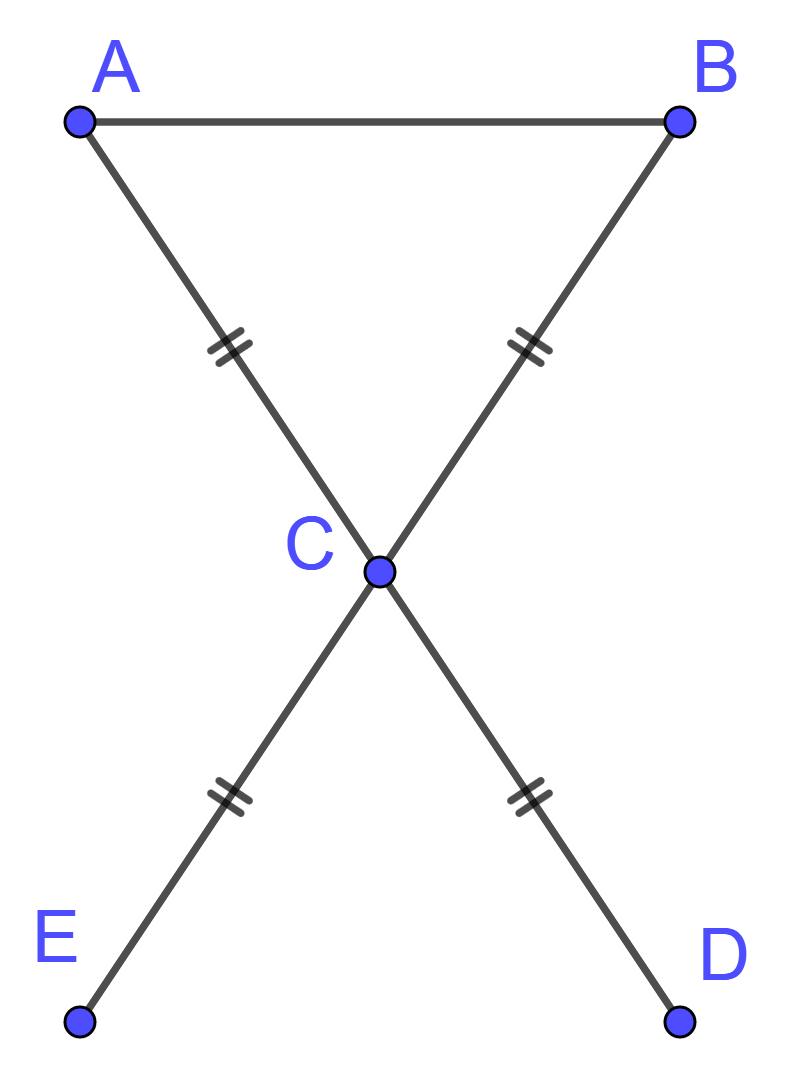
\includegraphics[scale=0.13]{img/tabouret}
\end{center}
	
	
\end{multicols}